\chapter{Domain Experts via Topic Modeling}

%\todo[inline]{Contains research questions for the experts; experimental setup; experimental results;summary}

\section{Introduction}

In this chapter, I address a problem which is analogous to the classic domain adaptation problem since the aim is to improve (morpho-)syntactic analysis for different domains, but more generic in nature. \textcolor{blue}{Classic domain adaptation assumes that there are two distinct data domains - source and target. However, often the source and the target contains a mix of domains, rather than a single one.} In order to simulate a more realistic scenario, I assume that the  dataset on which the taggers and the parsers is trained on, does not come from a single domain but may contain a mix of different domains. \textcolor{blue}{E.g., Wall Street Journal consists of news articles spanning various topics such as politics, finance, theatre critique, to name a few.}The same is true for the sentence that is parsed (or tagged) using the model trained on this dataset. I.e., the test sentence could potentially come from any of the domains. Thus, in my case, the problem is two fold - identify domains automatically in the training dataset and then suitably adapt the method to parse sentences more accurately. There is no manual work involved. 

I describe my method for improving POS tagging and dependency parsing for such heterogeneous datasets from a variety of different genres by creating experts for automatically detected topics. In this case, the datasets consist of newspaper reports on the one hand and biomedical extracts on the other. I assume that the domains have an equal participation in the dataset. \textcolor{blue}{Structuring the dataset in this way enables me to simulate the following:}
\begin{enumerate}
    \item  \textcolor{blue}{I am creating a dataset consisting of two specific and distinctive domains.}
    \item  \textcolor{blue}{Since I handcraft this dataset, I have a definite idea about the domain of each sentence.}
\end{enumerate}
I use Latent Dirichlet Allocation (LDA) to determine the topic of a sentence. LDA displays the latent topic structure in a document. In this case, a document to be clustered consists of a single sentence. I then assign each sentence to the most likely topic, for both training and test sentences. I train an expert for each topic and then use this expert to POS tag and parse the test sentences belonging to this topic. Note that, I use the term ``topic" in a slightly different sense than the topic modeler. I assume that the topics detected by the topic modeler do not only pertain to lexical differences, which can be beneficial for the POS tagger and the parser, but also to syntactic phenomena. Thus, one topic may focus on ``incomplete" sentences, such as headlines in a newspaper. It can also encapsulate certain nuances of a genre. E.g., one topic might show strong probability towards sentences containing political news. Another topic could be focused on sentences pertaining to different kinds of protein structures in DNA. 

The rest of the chapter is structured in the following way: \atrcomments{TBD after completion}


\section{Research Questions}\label{sec:quest}

\textcolor{blue}{POS tagging and dependency parsing tend to perform poorly on heterogeneous datasets, i.e., datasets consisting of sentences from different genres. This is mainly because of the different morpho-syntactic nature of the domains. Consider that we are training our tagger/parser on data consisting of sentences from newspaper domain and another widely different domain, such as conversation texts or biomedical abstracts. The syntactic nature of the sentences is distinctive. When the tagger/parser is trained on this, there are ample chances that the resulting training model will misidentify new sentences as belonging to a different domain and hence tag/parse inaccurately. The effective way could be to extend the training process and aid the tagger/parser in recognizing the domains. Thus, my goal is to create POS tagging and parsing experts for each of these genres/domains, which are present in the dataset. Given a mixed dataset, I create training experts which can effectively tag/parse new sentences. The idea is that, if we encounter a dataset with a mixture of domains, we can effectively determine the domains. Once the domains are identified, we can then create training models from these sentences. Thus, we have representative sentences and therefore training models for each domain. }
For example, the dataset might be a mixture of newspaper articles, blogs, financial reports, research papers and even specialized texts such as biomedical research papers and law texts. I create experts such that each expert would learn specific information about its own genre. I determine these experts by performing topic modeling on sentences and then train an expert on the sentences of the topic. I group sentences based on their most probable topic. To test the hypothesis that topic modeling can serve to group sentences into topics, I create a mixed dataset from the financial domain (using the Penn Treebank \cite{marcus:kim:ea:94}) and from the biomedical domain (using the GENIA Corpus \cite{tateisi:tsujii:04}) such that the new handcrafted corpus consists of sentences from both domains in equal measure. Consequently, there is a clear difference in the genres in the corpus, and I have gold standard topic information.

In this chapter, I investigate the possibility of creating genre experts, given a heterogeneous dataset. Thus, I perform topic modeling on training and test data simultaneously: I assign a test sentence to the topic with the highest probability. This means that I currently simplify the problem of assigning new sentences to topics. In the next chapter, I assign new sentences to topics based their similarity to sentences in the topics created during training, following the work by \citep{plank2011effective}. 

To summarize, I present the results on the following research questions in this chapter.

\subsection*{Question 1: Can topic modeling successfully identify genres in a dataset?} \label{q1}

%\atrcomments{need to remove WSJ ones for now}

\blue{In this question, my goal is to determine whether topic modeling can indeed identify the hidden genres/domains in a text. Suppose, we mix two domains to create a dataset and then run the topic modeler on this. It is then important to note whether the ``topics" given by the topic modeler are strongly indicative of the domains/genres. Thus one topic should predominantly contain sentences from first domain and the other topic should consist of sentences from the second domain. I.e., I estimate whether the data splits obtained from the topic modeler are meaningful for creating domain experts.
%In this question, I determine whether the data splits obtained from the topic modeler are meaningful for creating domain experts. I.e., I investigate whether an unsupervised topic modeler can detect topics in a heterogeneous corpus (table~\ref{tab:mixeddata}). 
%I mix two different corpora - news reports and biomedical abstracts - 
I assume if I mix two different corpora in equal measure, I can take their original corpus as gold standard.
%I use an artificially created heterogeneous corpus containing sentences from the Wall Street Journal (WSJ) section of the Penn Treebank \citep{marcus:kim:ea:94} and  from the GENIA Corpus \citep{tateisi:tsujii:04} and take their original corpus as the gold standard topic. 
The assumption is that a good split into the known topics, e.g.,  financial news and biomedical abstracts, will also improve POS tagging and parsing accuracy. 
If I assume two topics, we should be able to see a clear distinction between the financial news and biomedical sentences. I.e., for each topic, I should have a clear correspondence of its sentences to either domain/genre. I thus calculate the percentage of sentences in a given topic that belong to one genre and expect that one topic should have a high percentage and the other one a low percentage. I also experiment with a larger number of topics, to see if I can profit from a finer grained topic definition. However, this advantage will be offset by a smaller training set since we split into more sets.
}
%\atrcomments{Needs parsing experiments/need to check in the results sheet if this is there}

%\atrcomments{REMOVE} The finer grained split could also potentially identify micro-genres within a genre. I.e., the primary assumption is that - there are two very different genres and the topic modeler should be able to identify this distinction. In my case, WSJ and GENIA are representative of corpora from two very different domains - newspaper and biomedical texts. However, often the distinction between genres could be subtle. In that case, it is imperative to check if topic modeler could also identify micro-genres, in addition to the broader classification. To investigate this, I exclusively use the WSJ data set. The hypothesis is that the WSJ corpus contains different newspaper sections, which may use different styles. Since there is no information available from the Penn Treebank about those section, I cannot evaluate how well the topic modeler splits the sentences into topics, but I can evaluate whether the POS tagging/\atrcomments{parsing} experts are successful in adapting to those micro-genres.



\subsection*{Question 2: Does POS Tagging Benefit from Using Topic Experts?}

\blue{In this chapter I explore the effects of creating domain experts to better the performance of POS tagging and parsing. I suggest ways of using topic modeling to effectively cluster sentences into domain experts. It is then important to experiment whether using domain experts actually improves the performance.
POS tagging is often considered as a solved problem for homogeneous datasets. However, there is no performance guarantee when it comes to domain adaptation. The problem is also evident when the dataset contains syntactically varying sentences. This is an important consideration since POS tagging serves as a precursor to a lot of tasks including dependency parsing. 

Thus, in this question, I examine whether the performance of POS tagging improves if we create experts based on the topics detected by the topic modeler.
In order to investigate this question, I generate a two-topic corpus by combining data from the Wall Street Journal (WSJ) section of the Penn Treebank \cite{marcus:kim:ea:94} and from the GENIA corpus \cite{tateisi:tsujii:04} as shown in table~\ref{tab:mixeddata}. The WSJ covers financial news while GENIA uses Medline abstracts as its textual basis. As a consequence, I have sentences from two different genres, but also slight variations in the POS tagsets. The tagset used in GENIA is based on the Penn Treebank tagset, but it uses the tags for proper names and symbols only in very restricted contexts. This setup allows me to test whether the topic modeler is able to distinguish the two genres, and whether POS tagging experts can profit from this separation. I assign sentences to topics based on the highest probability exhibited by the topic modeler. I then train a POS tagging expert on the training part of each topic. I then use the expert to tag the test sentences from this topic. In this setting, we can see if the experts can effectively handle the data sparseness caused by dividing the training set into multiple experts. Thus, I experiment with the setting in which I use topic modeling as hard clustering i.e., I assign each sentence to the topic for which the topic modeler gave the highest probability. 
%In a second setting, I experiment with soft clustering. I.e., I add  each sentence to all topics, weighted by its probability distribution.
}
%\textcolor{red}{I could also potentially experiment with a different clustering technique - soft clustering, in which I add  each sentence to all topics, weighted by its probability distribution. I discuss these clustering techniques in more detail in the next section}
%I also experiment with soft clustering, in which I add each sentence to all topics, weighted by its probability distribution.

\subsection*{Question 3: Does Dependency Parsing Benefit from the Topics Experts?}

\blue{Domain adaptation is a considerably challenging problem for dependency parsing. The problem is still sizeable for heterogeneous datasets because in addition to classic domain adaptation, we are dealing with an added problem of identifying underlying domains\todo{really?}. 
Here, I investigate the effects of using topic modeling experts for dependency parsing. I use hard clustering i.e., assigning sentences to experts based on the highest probability topic given by the topic modeler. Initially, I use gold POS tags in order to abstract away from POS tagging quality. In a second step, I investigate the interaction between POS tagging and parsing experts. I.e., I am interested in whether dependency parsing can profit from using the POS tags that were determined by the POS tagging experts. This helps in determining whether integrating POS information given by the POS experts can improve dependency parsing or whether there is no interaction between the two levels. 
}

%Similar to POS tagging experts, I experiment with two different clustering techniques - hard \& soft clustering to address the data sparsity issue.

\subsection*{Question 4: How do we cluster sentences into experts?}


% The experts can be determined based on hard or soft clustering decisions: For hard clustering, the sentences are assigned to hard topics, based on the topic that has the highest probability in that sentence. I.e., if for sentence $s_x$, MALLET lists the topic $t_1$ as the topic with the highest probability, then $s_x$ is added to the data set of topic $t_1$. In other words, the data set of topic $t_1$ consists of all sentences for which MALLET showed topic $t_1$ as the most likely topic. This means that the data set sizes vary between topics. This is a simplification since a sentence can represent different topics to different degrees. Thus, I investigate whether I can utilize the soft clustering information directly and add every sentence to every POS tagging expert, weighted based on the degree to which it represents the topic of this expert. This not only allows me to model topics in more detail, it can also help combating data sparsity since every sentence contributes to every domain expert.

% Hence, for soft clustering experiments, I utilize the entire topic distribution of a sentence by weighting sentences in the training data based on their topic distribution. I simulate weighting training sentences by adding multiple copies to the training files of the experts. Thus, for 2-topic experiments, a sentence with 80\% probability for topic~1 will be included 8 times in the expert for topic~1 and 2 times in the expert for topic~2, rounding up small percentages so that every sentence will be added to every expert at least once.  Thus, I use a more fine grained topic model while mitigating data sparseness,  but we risk adding non-typical / irrelevant sentences to experts.

\blue{In the previous questions, I looked at creating POS tagging and dependency parsing experts using a hard clustering approach. However, this technique assumes that we assign sentences to the highest probability topic. 
I.e., the sentences are assigned to hard topics, based on the topic that has the highest probability in that sentence. I.e., if for sentence $s_x$, MALLET lists the topic $t_1$ as the topic with the highest probability, then $s_x$ is added to the data set of topic $t_1$. In other words, the data set of topic $t_1$ consists of all sentences for which MALLET showed topic $t_1$ as the most likely topic. This means that the data set sizes vary between topics. 
%This is a simplification since a sentence can represent different topics to different degrees.
We are essentially dividing the dataset into the fraction of number of topics. Thus, creating experts causes an inherent data sparsity. Moreover, having a finer grained split, i.e., larger number of topics could result in severe data sparseness. 
%This is assuming that we treat topics as hard clusters, i.e., every sentence belongs to the topic with the highest probability. 
In addition to the data sparsity issue, the hard clustering assumption is also a simplification since a sentence can represent different topics to different degrees. This is especially true in case of identifying micro-genres or larger number of topics, in general. 
A potential solution is to investigate whether we can utilize the entire topic probability distribution for a sentence.
%soft clustering information directly and 
I.e., I add every sentence to every domain expert, weighted based on the degree to which it represents the topic of this expert. I will refer to this method as soft clustering. I simulate weighting training sentences by adding multiple copies to the training files of the experts. This not only allows me to model topics in more detail, it can also help combating data sparsity since every sentence contributes to every expert. Thus, for 2-topic experiments, a sentence with 80\% probability for topic~1 will be included 8 times in the expert for topic~1 and 2 times in the expert for topic~2, rounding up small percentages so that every sentence will be added to every expert at least once.  Thus, I use a more fine grained topic model while mitigating data sparseness,  but we risk adding non-typical / irrelevant sentences to experts. I.e., I ``diffuse'' the expert knowledge too much by adding all sentences even if they are weighted. 

It is important to consider the trade-offs between the clustering methods. Both of these methods have their pros and cons in different situations. 
My hypothesis is that, in cases where the domain split is clear and definite, hard clustering could potentially be a better choice than soft clustering, even at the risk of data sparsity caused by dividing the training set. I.e., If I create 10 experts, I am basically dividing the training set to a fraction of 10. This essentially means that, now my training experts can only train on $\frac{1}{10}^{th}$ of the full training set. 

\todo{overkill?}However, there are sentences which could be ambiguous in terms of domain. In this case, soft clustering will be a better approach to take. This is because, we are not at risk of losing information by considering the highest probability topic and ignoring others. Hence, it will be interesting to observe whether adding more training data using soft clustering can actually improve the overall performance. 

% In the research questions, I outlined a setting of using a finer grained split with a larger number of topics. However, evidently, %mentioned that having a finer grained split, i.e., 
% larger number of topics could result in severe data sparseness. This is assuming that I treat topics as hard clusters, i.e., every sentence belongs to the topic with the highest probability. So,creation of experts causes a sparsity in the training data because I am dividing the training set into a number of experts. 
% I demonstrate the hypothesis with an example. 
% This is also a simplification since a sentence can represent different topics to different degrees. This is especially true in case of identifying micro-genres or larger number of topics, in general.
Consider the following example:

In order to represent the distinct domains (WSJ, GENIA) and also the sub-genres of a particular domain, I create 2 as well as 10 topics experts. Typically, if I consider the topic prior as 2 \& 10, the distribution looks as given in Table~\ref{tab:2topicssent} \& \ref{tab:10topicssent}~\footnote{an approximation}, for the following WSJ sentence:

``Though growers can't always keep the worm from the apple , they can protect themselves against the price vagaries of any one variety by diversifying -- into the recently imported Gala , a sweet New Zealand native ; the Esopus Spitzenburg , reportedly Thomas Jefferson's favorite apple ; disease-resistant kinds like the Liberty."
 
 % Please add the following required packages to  document preamble:
%\usepackage{multirow}
\begin{table*}[!htb]
\centering

\caption{2 topics distribution}
\begin{tabular}{cc}
%\multicolumn{2}{c}{2-topic probability distribution} 
\\ \hline
0 & 1 \\
95.90 & 4.10 \\ \hline
\end{tabular}
\label{tab:2topicssent}

\caption{10 topics distribution
%\\ 
}
\begin{tabular}{cccccccccc}
%\multicolumn{10}{c}{10-topic probability distribution} 
\\ \hline

0 & \multicolumn{1}{c}{1} & \multicolumn{1}{c}{2} & \multicolumn{1}{c}{3} & \multicolumn{1}{c}{4} & \multicolumn{1}{c}{5} & \multicolumn{1}{c}{6} & \multicolumn{1}{c}{7} & \multicolumn{1}{c}{8} & \multicolumn{1}{c}{9} \\
0.11 & 0.10 & 0.08 & 0.10 & 0.09 & 30.58 & 15.28 & 49.55 & 3.93 & 0.16 \\ \hline
\end{tabular}
\label{tab:10topicssent}

%\caption{2 \& 10-topic probability distribution for a WSJ corpus sentence: \\ }
%\label{tab:10t-probab}
\end{table*}
 
In Table~\ref{tab:2topicssent} and~\ref{tab:10topicssent}, we can see the probability of the highest (7) and the second highest (5) topic are fairly close. Thus, if I take topic 7 and discard the other topics, I lose a fair share of information given by LDA. In other words, dividing a corpus into experts creates a significant sparsity in training data if I consider the highest probability topic and discard the rest.
This problem can be mitigated if we effectively utilize the whole topic probability distribution by giving a sentence to more than one topic. Thus, I also investigate whether we can utilize the soft clustering information directly and add every sentence to every domain expert, weighted based on the degree to which it represents the topic of this expert. This not only allows us to model topics in more detail, it can also help combating data sparsity since every sentence contributes to every expert. The risk is that I diffuse the expert knowledge too much by adding all sentences even if they are weighted. 
}

\subsection*{Question 5: What do the Experts Learn?}

\blue{
In the previous questions, I described my hypothesis on creating experts for POS tagging and dependency parsing. POS tagging and dependency parsing has certain known issues in domain adaptation situation. Thus, evaluating the results on these issues, will help ascertain the source of improvements as a result of using the domain experts. Thus, in this question, I take a closer look at the results from the previous question to learn where the improvements by the experts (POS tagging \& parsing) come from. }
    %I investigate on certain known issues for both POS tagging and dependency parsing in domain adaptation situation and in general, to ascertain the source of these improvements. 

For POS tagging, out of vocabulary words are a major concern. Hence, I analyze whether all the improvements based on lower rates of out-of-vocabulary words. For example, suppose we have two experimental settings, both using the same size of the training set, but in one setting, the majority of the training set is from GENIA while in the second setting, the training set is a mix of GENIA and WSJ. It is more likely that the former will contain a wider range of biomedical vocabulary than the latter. However, it is also possible that the experts will learn different regularities, for example with regard to how the proper name tags are used in the two corpora. Thus, I look at the ratio of unknown words in the different experiments and at the error rates of known and unknown words. I additionally look at the confusion matrices.

I also analyze the parsing results in more detail to gauge the effect of using topic modeling experts. Here, I'm primarily interested in whether there are specific types of sentences or dependencies that are grouped by the topic models, so that the parsing experts focus on a specific subset of syntactic properties. Genre differences can be captured by adapting to certain syntactic phenomena. Hence, I look more closely if there is a particular type of sentence that benefit from using experts over the general case. Mislabeling of dependency is another problem, which can impact overall performance of the parser. I look at confusion matrices for dependency labels to further investigate if there is an improvement from using the experts. 

\section{System Overview}\label{sec:setup}

\subsection{Architecture}

\begin{figure*}[!htb]
    \centering
    \includegraphics[width=\textwidth]{figures/approach.png}
 \caption{Overview of the architecture of the POS tagging and parsing experts.}\label{fig:architecture0}
 \end{figure*}

Figure~\ref{fig:architecture0} shows the overall architecture of the system. 
I use sentences as documents. Note that, I utilize the artificial heterogeneous WSJ+GENIA corpus, described in section~\ref{sec:wsjgeniamixedcorpus}. Topic modeling shows the distribution of topic probabilities for every sentence. Thus, if we have $n$ topics, we get a probability distribution for $n$ topics for a particular sentence. Based on this topic probability distribution, I group sentences into sentence clusters. These sentences are representative of the genres/domains. I create training models (for both POS tagging and dependency parsing) from these sentences, which can then be regarded as ``experts" for a particular genre/domain. For tagging/parsing a sentence from the test dataset, I re-execute the topic modeler to determine which domain/genre the sentence belongs to. This method of rerunning the topic modeling can be expensive and hence I devise a method to effectively address this problem in the next chapter. Once this sentence is assigned to a cluster, I use the training model for that cluster to tag/parse that sentence.

%Based on the document topic information, I then group the sentences into genre topics. 
%Note that, I utilize the artificial heterogeneous WSJ+GENIA corpus, described in section~\ref{sec:wsjgeniamixedcorpus}. I collect all sentences from the training and test set, cluster them via the MALLET topic modeler, and determine for which expert(s) the sentence is relevant to. There are several ways of determining the best expert based on the probability distribution of topics in a sentence. Then, we separate the sentences for each expert into training and test sentences, based on the previously determined data splits (see above).



%\subsection{Clustering Decision} 
%\todo[inline]{Not sure if this should be here or in a separate chapter or a research question}



\subsection{Baselines}

I define two baselines to compare my results with. As the first baseline, I take the complete training set when no topic modeling is performed. Note that this is a very competitive baseline since the topic modeling experts have access to considerably smaller amounts of training data.  In order to avoid differences in accuracy resulting from different training set sizes, I create a second baseline by splitting the sentences randomly into the same number of groups as the number of topics, while maintaining the equal distribution of WSJ and GENIA sentences where applicable. I.e., I assume the same number of random ``topics'', all of the same size. Thus, in the 2-topic setting with the the genres, I create two separate training sets, each containing half of the WSJ training set and half of the GENIA one. In this setting, I test all experts on the whole test set and average over the results.

% \subsection{Evaluation}

% I use the script \texttt{tnt-diff} that is part of TnT to evaluate the POS tagging results  and the CoNLL shared task evaluation script\footnote{http://ilk.uvt.nl/conll/software/eval.pl} for evaluating the parsing results. I report the overall accuracy for POS tagging and attachment scores (labeled \& unlabeled) for dependency parsing.
% I report the following evaluation metrics for evaluation:

% \begin{itemize}
%     \item POS tagging
%     \begin{itemize}
%         \item Overall Accuracy: For POS tagging, we evaluate the results based on the accuracy of identifying POS tags correctly in the test set as shown in~\ref{eq:posacc}. I.e., we measure how many tags have been correctly identified in the test set.
%         \begin{equation} \label{eq:posacc}
%             Accuracy = \frac{Number\ of\ correctly\ identified\ tokens}{total\ number\ of\ tokens}
%         \end{equation}
%         \item Accuracy for Known \& Unknown tokens: For POS tagging, unknown or out of vocabulary words (OOV) pose as a challenging problem. \texttt{tnt-diff} provides an utility to measure accuracy based on number of correct predictions for known vs. unknown words. I discuss the method employed by TnT to determine the POS tags for unknown words in chapter \atrcomments{TBD}. I.e., we can determine the accuracy on known and OOV words separately. Since performance on OOV words is an essential determining factor, I use this metric to further analyze the results from domain experts in greater detail. This is a bigger challenge in a domain adaptation situation since there are domain specific words for each domain, which tend to get misclassified in a heterogeneous dataset.
%     \end{itemize}
%     \item Dependency Parsing
%     \begin{itemize}
%         \item Labeled Attachment Scores (LAS): For evaluating the results of dependency parsing experiments in this chapter, I report LAS\footnote{I report micro-averaged LAS. Micro-averaged LAS is reported on words as opposed to macro-averaged LAS, which considers sentences as the grain.}.  As \ref{eq:las} shows, LAS estimates the number of words with correctly predicted head and label.
%         \begin{equation} \label{eq:las}
%             LAS = \frac{number\ of\ words\ with\ correct\ head\ and\ label}{total\ words}
%         \end{equation}
        
%         \item Unlabeled Attachment Scores (UAS): UAS, as the name suggests, evaluates based on correctly predicted head. 
%         \begin{equation} \label{eq:uas}
%             UAS = \frac{number\ of\ words\ with\ correct\ head}{total\ words}
%         \end{equation}
        
%     \end{itemize}
% \end{itemize}



\section{Experimental Results}\label{sec:results}


In this section, I discuss the results of the experiments based on the research questions delineated in section~\label{sec:quest}.

\subsection*{Question 1: Can topic modeling successfully identify genres in a dataset?}

\begin{figure*}[!t]
    \centering
    \fbox{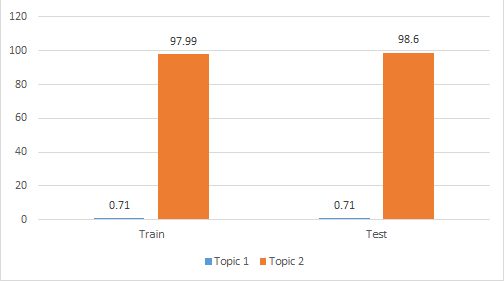
\includegraphics[width=\textwidth]{figures/dist-sent-2.png}}
 \caption{Distribution of GENIA sentences in 2-topic experts.}\label{fig:distsent2}
 \end{figure*}
 
 
 
 
 \begin{figure*}[!t]
    \centering
    \fbox{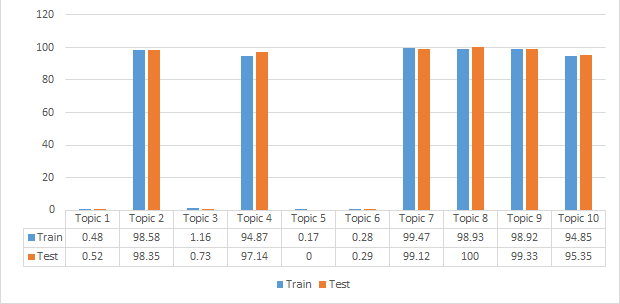
\includegraphics[width=\textwidth]{figures/dist-sent-10.png}}
 \caption{Distribution of GENIA sentences in 10-topic experts.}\label{fig:distsent10}
 \end{figure*}

%\todo[inline]{Based on EACL split}

\begin{table}[t!]
	\begin{center}
		\begin{tabular}{r|rr|rr} 
			& \multicolumn{2}{c|}{2 topics} & \multicolumn{2}{c}{10 topics}\\
			T. &\% in train & \%in test & \% in train & \% in test \\ 
			\hline
			1 	& 0.71	& 	0.71 	& 0.48 	& 0.52		\\ 
			2 	& 97.99	& 	98.6	& 98.58 	& 98.35				\\
			3 	& 		& 			& 1.16 	& 0.73			\\ 
			4 	& 		& 			& 94.87	& 97.14		\\
			5 	& 		& 			& 0.17	& 0			\\  
			6 	& 		& 			& 0.28 	& 0.29				\\  
			7 	& 		& 			& 99.47	& 99.12			\\  
			8 	& 		& 			& 98.93 	& 100		\\ 
			9 	& 		& 			& 98.92	& 99.33			\\ 
			10 	& 		&			& 94.85 	& 95.35			\\   
			\hline 
		\end{tabular}
	\end{center}
	\caption{Distribution of sentences from the WSJ+GENIA data set given 2 and 10 topics (showing the percentage of GENIA sentences per topic).\label{tab:cluster}}
\end{table}

Following question 1, I investigate whether LDA can separate the sentences into meaningful topics. 
Figures~\ref{fig:distsent2} and \ref{fig:distsent10} shows the distribution of GENIA sentences for 2 \& 10 topic experts. These results indicate that the topic modeler effectively separates topics.For the 2-topic case (figure~\ref{fig:distsent2}), a clear split is evident as the majority of the GENIA sentences are clustered in topic 2. The percentage of GENIA sentences clustered in topic 1, is less than 1\%. Thus, the rate is misclassification is extremely low, proving that this is a viable way to determine genre distinction. Table~\ref{tab:misclassifiedsent} shows some examples of WSJ sentences misclassified as GENIA and viceversa for the 2-topics case. Additionally, table~\ref{tab:ex:2topics} shows example words from the 2-topic experiment, which show a clear separation of topics into biomedical and financial terms.
%\todo{describe more may be?}
%Table~\ref{tab:cluster} shows the distribution of sentences in the training and test set into different topics when I assume 2 or 10 topics. 
% ; the misclassified sentences constitute less than 1\%. Table~\ref{tab:misclassifiedsent} shows examples of a GENIA sentences misclassified as WSJ sentence and vice versa.%\todo[inline]{insert a misclassification example here; write a little bit about it}

\begin{table}[!htb]
\begin{tabular}{c|c|l}
\begin{tabular}[c]{@{}c@{}}Gold\\ Label\end{tabular} & \begin{tabular}[c]{@{}c@{}}Classified\\ Label\end{tabular} & \multicolumn{1}{c}{Sentences} \\ \hline
WSJ & GENIA & \begin{tabular}[c]{@{}l@{}}The  Diet  plays  a  minor  role  compared  with  the  powerful  bureaucratic \\ system.\end{tabular} \\
WSJ & GENIA & "I tried." \\ \hline
GENIA & WSJ & Copyright 1997 Academic Press. \\
GENIA & WSJ & But many puzzles of the drugs remain. \\ \hline
\end{tabular}
\caption{Misclassified sentences}
\label{tab:misclassifiedsent}
\end{table}

\begin{table}[!htb]
	\begin{tabular}{l|p{14cm}} 
	    1 & mr million ui year company market stock billion share corp years shares trading president time quarter sales government business \\ \hline 
		2 & cells cell expression il nf activation human binding gene  transcription protein kappa ab cd ti factor alpha activity induced     \\ \hline
		
	\end{tabular}
	\caption{Examples of words in topics for the 2-topic experiments on the WSJ+Genia corpus.}
	\label{tab:ex:2topics}
\end{table}

Figure~\ref{fig:distsent10} shows topic-wise distribution of GENIA sentences for train as well as test dataset for the 10-topic experiments. We notice that topics 2, 4, 7, 8, 9, and 10 contain mainly GENIA sentences while the remaining topics cover mainly WSJ sentences. In both settings, the error rate is between 0.2\% and 5\% (see table~\ref{tab:cluster}), i.e., I obtain a distinct split between GENIA and WSJ, which should give us a good starting point for creating POS tagging and dependency parsing experts. 




\subsection*{Question 2: Does POS Tagging Benefit from Using Topics?}

\begin{table}[t]
\centering
\begin{tabular}{l|cc}
 & \multicolumn{2}{c}{Accuracy} \\
Setting & \multicolumn{1}{r}{2 topics} & \multicolumn{1}{r}{10 topics} \\ \hline
Full training set & \multicolumn{2}{c}{96.64} \\
Random split & 96.48 & 95.49 \\
Topic model & \textbf{96.84} & 96.34 \\ \hline
%Soft Clustering & 96.73 & \textbf{96.84} \\ \hline
\end{tabular}
\caption{Comparing the topic model experts to the baselines on the WSJ+GENIA data set.\label{tab:mixedresults}}
\end{table}


In this section, I discuss the results on the experiments for question whether the POS tagger can benefit from using topic modeling, i.e., whether POS tagging results can be improved by training experts for genres provided by topic modeling. I compare the topic modeling approach to  two baselines for the 2-topic and 10-topic setting. %I also perform a soft clustering experiment, in which each sentence is added to every topic, weighted by its probability.

The results in Table~\ref{tab:mixedresults} show that if I assume a 2-topic setting, the experts perform better than both baselines, i.e., the model trained on the full training set and the model with randomly chosen ``topics". The 2-topic expert model reaches an accuracy of 96.84\%, which is slightly higher than the full training set accuracy of 96.64\%. We know that the 2-topic setting provides a clear separation between WSJ and GENIA (Table~\ref{tab:cluster}). Thus, this setting outperforms the full training set using a smaller amount of training data. There is also an increase of 0.36 percent points over the accuracy of the 2 random split setting. 

For the 10-topic setting, the topic expert model outperforms the random split of the same size by 0.85 percent points, which is a higher difference than for the 2-topic setting. This shows that the finer grained  splits model important information. However, the topic expert model does not reach the accuracy of the baseline using the full training set. This can be attributed to the reduced size of the training set for the experts. The experts encounter around $\frac{1}{10}/$ of the training data as compared to the full training baseline and this data sparseness causes a drop in performance.


%Since training set size is a detrimental factor for the larger number of topics, I also conducted an experiment where I use soft clustering so that every sentence is represented in every topic, but to a different degree. The last row in table~\ref{tab:mixedresults} reports the results of this experiment. We notice that the 2-topic experts cannot benefit from the soft clustering. Since the separation between WSJ and GENIA is very clearly defined for the 2-topic experiments,  the advantage of having a larger training set is outweighed by too many irrelevant examples from the other topic. However, the 10-topic model profits from the soft clustering, which indicates that soft clustering can alleviate the data sparseness problem of the POS tagging experts for larger numbers of topics. 

%A more detailed analysis of the POS tagging results (on a slightly different data split), see \cite{mukherjee:kuebler:ea:16}. This work includes an experiment showing that the POS tagging experts also increase performance for the WSJ corpus only, showing that POS tagging experts also perform better on more homogeneous collections, i.e., they adjust to less obvious differences between sentences.

%\subsection{Parsing Experts}

\subsection*{Question 3: Does Dependency Parsing Benefit from the Topics?}

In this section, I present the results of using topic experts for dependency parsing. I discuss my results from two perspectives. One, where I assume I have gold POS tags and another, where I use POS tags from TnT as an input to the parser. This will help me in determining the effect of POS tags on parsing choices. 

\subsubsection*{Using Gold POS Tags}\label{sec:goldpos}

\begin{table*}[t!]
	\centering
	\begin{tabular}{l|cc|cc}
		\multicolumn{1}{c|}{\multirow{2}{*}{Setting}} & \multicolumn{2}{c|}{LAS}                                      & \multicolumn{2}{c}{UAS}                                     \\
		\multicolumn{1}{c|}{}                         & \multicolumn{1}{l}{2 topics} & \multicolumn{1}{r|}{10 topics} & \multicolumn{1}{l}{2 topics} & \multicolumn{1}{r}{10 topics} \\ \hline
		Full training set                             & \multicolumn{2}{c|}{88.67}                                    & \multicolumn{2}{c}{91.71}                                   \\
		Random split                                  & 87.84                        & 84.91                          & 90.86                        & 88.64                         \\
		Topic model                                   & \textbf{90.51}               & 88.38                          & \textbf{92.14}               & 90.3                          \\ \hline
		%Soft clustering                               & 89.86                        & \textbf{89.91}                 & 91.99                        & \textbf{91.84}                \\ \hline
	\end{tabular}
	\caption{Results of the dependency parsing experiments using gold POS tags.}
	\label{tab:tmvsfs}
\end{table*}

I now look into the parsing experiments using gold standard POS tags. The choice of gold POS tags allows me to focus on the contribution of the topic modeling experts on parsing results mainly while abstracting away the effect of POS tags on parsing decisions. 

The results of the experiments are shown in Table~\ref{tab:tmvsfs}, for 2-topic and 10-topic settings and in comparison to the two baselines for hard clustering i.e., taking the highest topic probability as the determining factor for cluster membership. %and soft clustering experiments. 
The hard clustering results indicate that the 2-topic expert model reaches an improvement over the baseline using the full training set for both the labeled attachment score (LAS) and the unlabeled attachment score (UAS). There is an increase of around 2\% over the baseline for LAS, and an increase of 0.43\% for UAS. However, for the 10-topic setting, both the LAS and the UAS are slightly lower than the baseline. For LAS, the difference is 0.29 percent points while for UAS, the difference is 1.41 percent points. This shows that the gain in LAS and UAS is offset by the reduced training set, parallel to the results for POS tagging. Both the 2-topic and the 10-topic experts outperform the random split baseline (which uses similar training set sizes), with a gain of more than 3 percent points.

%The soft clustering results show the same trends as in the POS tagging experiments:  For the 2-topic setting, soft clustering outperforms the full baseline by 1.19 percent points. But it does not exceed the hard clustering results.  In the 10-topic setting, soft clustering outperforms the full baseline as well as the hard clustering setting. This is because sentences with a 50\% probability of belonging to topic~1 and a 40\% probability for topic~3 need to be considered to belong to both topics. This result also shows that this method effectively handles the training data sparsity in the 10-topic setting.


\begin{table*}[t!]
	\centering
	\begin{tabular}{l|rr|rr}
		\multicolumn{1}{l|}{\multirow{2}{*}{Setting}} & \multicolumn{2}{c|}{LAS} & \multicolumn{2}{c}{UAS} \\
		\multicolumn{1}{c|}{} & 2 topics & 10 topics & 2 topics & 10 topics \\ \hline
		1. Full set POS + full set parsing & \multicolumn{2}{c|}{86.70} & \multicolumn{2}{c}{90.26} \\ 
		2. Random split POS + random split parsing & 85.77 & 81.33 & 89.11 & 85.73 \\ 
		3. Full set POS + topic model parsing & 88.30 & 86.13 & 90.43 & 88.47 \\ 
		4. Topic model POS + Topic model parsing & \textbf{88.35} & 85.68 & \textbf{90.55} & 88.15 \\ 
		\hline
	\end{tabular}
	\caption{Results of the dependency parsing experiments using TnT POS tags.}
	\label{tab:TnTPOS}
\end{table*}



\subsubsection*{Using the POS Tagger}\label{TnTPOSinParsing}

In this section, I explore the results of using POS tags from the POS tagger TnT as the input for the parser. Thus, in this case, I consider the effects of POS tags on parsing decisions. This gives rise to four major scenarios:

\begin{enumerate}
	\item The full training set is used for POS tagging and for parsing (full baseline). In this case, I train the POS tagger on the full training set and then use these POS tags for parsing. The parser also has access to the full training set. This enables me to draw a parallel baseline to the original full training baseline.
	\item Random splits are used for parsing and POS tagging. I.e., the POS tagger and parser are trained on random splits (random baseline). This is similar to the full training set baseline, except I use random splits for POS tagging and these tags are incorporated in parsing. 
	\item Topic models are used for training the parser, but TnT is trained on the whole training set. In this case, I abstract the effect of using topic modeling experts on POS tags. I.e., I evaluate the performance based on POS tags trained on the full training set. The parser, however, is trained on the experts which uses these POS tags.
	\label{S2}
	\item Topic models are used for training the parser and the POS tagger. For this scenario, I assess the effect of using POS tags determined by the POS experts in the parsing experts. \label{S1}
\end{enumerate}

I use the random split case as the lower baseline for these experiments and the full training set as the more competitive baseline. Table~\ref{tab:TnTPOS} shows the results.


Table~\ref{tab:TnTPOS}  shows that in the 2-topic setting, using topic modeling experts on the POS level as well as on the parsing level reaches the highest results with an improvement of around 2\% in LAS in comparison to the full baseline parser, from 86.70\% to 88.35\%. The gain in UAS is considerably smaller: The topic modeling expert reaches 90.55\% as opposed to 90.26\% for the full baseline. In contrast, the topic modeling setting for the 10-topic setting outperforms the random baseline but does not reach the full baseline,  thus mirroring the trends we have seen before.



When I compare the experiments where I use the full POS tagging baseline along with topic model parsing experts (row 3 in table~\ref{tab:TnTPOS}) to the full topic model (row 4), I observe that the latter model reaches only very minimal gains by using the topic modeling POS tagger when I use 2 topics, and there is a negative trend when I use 10 topics. I.e. the overall quality of the POS tagger is more important than its specialization. Thus, even if the topic model POS tagger outperforms its full baseline, the learned adaptations only have a minimal effect on parsing accuracy.

\subsection*{Question 4: How do we cluster sentences into experts? }

\begin{table}[t]
\centering
\begin{tabular}{l|cc}
 & \multicolumn{2}{c}{Accuracy} \\
Setting & \multicolumn{1}{r}{2 topics} & \multicolumn{1}{r}{10 topics} \\ \hline
Full training set & \multicolumn{2}{c}{96.64} \\
Random split & 96.48 & 95.49 \\
Topic model & \textbf{96.84} & 96.34 \\ 
\textbf{Soft Clustering} & 96.73 & \textbf{96.84} \\ \hline
\end{tabular}
\caption{Soft Clustering for POS tagging experts.\label{tab:poswsoftcluster}}
\end{table}

In the previous questions, I discussed creating experts for POS tagging and parsing using the highest probability topic as the guiding factor in deciding which cluster a sentence belong to. However, the finer grained split into topics causes severe data sparsity for hard clustering. The training set size is actually a detrimental factor for the larger number of topics. Hence, I conduct experiments for POS tagging and parsing, where I use soft clustering so that every sentence is represented in every topic, but to a different degree. The last row in table~\ref{tab:poswsoftcluster} reports the results of this experiment. We notice that the 2-topic experts cannot benefit from the soft clustering. Since the separation between WSJ and GENIA is very clearly defined for the 2-topic experiments,  the advantage of having a larger training set is outweighed by too many irrelevant examples from the other topic. However, the 10-topic model profits from the soft clustering, which indicates that soft clustering can alleviate the data sparseness problem of the POS tagging experts for larger numbers of topics. 

\begin{table*}[t!]
	\centering
	\begin{tabular}{l|cc|cc}
		\multicolumn{1}{c|}{\multirow{2}{*}{Setting}} & \multicolumn{2}{c|}{LAS}                                      & \multicolumn{2}{c}{UAS}                                     \\
		\multicolumn{1}{c|}{}                         & \multicolumn{1}{l}{2 topics} & \multicolumn{1}{r|}{10 topics} & \multicolumn{1}{l}{2 topics} & \multicolumn{1}{r}{10 topics} \\ \hline
		Full training set                             & \multicolumn{2}{c|}{88.67}                                    & \multicolumn{2}{c}{91.71}                                   \\
		Random split                                  & 87.84                        & 84.91                          & 90.86                        & 88.64                         \\
		Topic model                                   & \textbf{90.51}               & 88.38                          & \textbf{92.14}               & 90.3                          \\ 
		\textbf{Soft clustering}                               & 89.86                        & \textbf{89.91}                 & 91.99                        & \textbf{91.84}                \\ \hline
	\end{tabular}
	\caption{Results of the dependency parsing experiments using gold POS tags.}
	\label{tab:parsingsoftcluster}
\end{table*}


Next, I investigate the effect of soft clustering on parsing experts. The soft clustering results show the same trends as in the POS tagging experiments:  For the 2-topic setting, soft clustering outperforms the full baseline by 1.19 percent points. But it does not exceed the hard clustering results.  In the 10-topic setting, soft clustering outperforms the full baseline as well as the hard clustering setting. This is because sentences with a 50\% probability of belonging to topic~1 and a 40\% probability for topic~3 need to be considered to belong to both topics. This result also shows that this method effectively handles the training data sparsity in the 10-topic setting.


\subsection*{Question 5: What do the experts learn?}

\begin{table*}[t!]
	\centering
	\begin{tabular}{p{11cm}|r|r}
		\multicolumn{1}{c|}{Sentence} & \multicolumn{1}{c|}{\begin{tabular}[c]{@{}c@{}}Fulltext\\ LAS\end{tabular}} & \multicolumn{1}{c}{\begin{tabular}[c]{@{}c@{}}2-topic \\ LAS\end{tabular}} \\ \hline
		Phyllis Kyle, Stephenson Newport News , Va . & 0 & 25.00 \\
		But volume rose only to 162 million shares from 143 million Friday . & 46.15 & 61.54 \\
		Fidelity , for example , prepared ads several months ago in case of a market plunge . & 47.06 & 82.35 \\
		CALL IT un-advertising . & 50.00 & 75.00 \\
		( See related story : " And Bills to Make Wishes Come True " -- WSJ Oct. 17 , 1989 . & 52.38 & 61.90 \\
		\hline
	\end{tabular}
	\caption{Comparison of LAS for the sentences with the lowest LAS in the fulltext setting.}
	\label{tab:compLASTMvsFS}
\end{table*}


\begin{table*}[t!]
\centering
\begin{tabular}{ll|rrr}

Gold Dep. & Pred. Dep. & Fulltext  &Topic~1  & Topic~2 \\ \hline
ADV & NMOD & 121 & 37 & 86\\
PMOD & NMOD & 101 & 21& 67\\
NMOD & ADV & 100 & 34 & 57 \\
AMOD & NMOD & 91 & 26 & 83\\
CONJ & NMOD & 86 & 13 & 56\\ \hline
\end{tabular}
\caption{The 5 most frequent dependency label confusions of the full baseline parser.}
\label{tab:conf:FT:TM}
\end{table*}

\todo[inline]{This could be like this or it could be 2 separate research question - one for POS tagging and one for parsing}

It is important to delve deeper into the results to understand where improvement stems from. For POS tagging, the experts outperformed the random split baseline by a greater margin. Hence I take a closer look at the differences. I analyze the results for gold POS tags experiments to better understand the improvement for dependency parsing, since it yields most accurate predictions.  

\begin{table*}[t]
	\begin{center}
	\resizebox{\textwidth}{!}{%
		\begin{tabular}{l|rrr|rrr} 
			& \multicolumn{3}{c}{Random split} & \multicolumn{3}{|c}{Topic model}\\
			Topic & \% Unknown & Known Acc.  & Unknown Acc. & \% Unknown & Known Acc. & Unknown Acc. \\
			\hline
			1 & 4.79 & 97.06 &  82.84 & 4.29 & 96.29 &  85.31 \\
			2 & 4.86 & 97.25&  83.38 & 3.85 & 98.35 &  85.12 \\ 
			
			 \hline 
			avg. & 4.83 & 97.16 & 83.11 & 4.07 & 97.33 & 85.22\\ \hline
		\end{tabular}%
		}
	\end{center}
	\caption{Unknown word rates and accuracies for known and unknown words in the WSJ+GENIA experiment using 2 topics.\label{tab:known}}
\end{table*}

\subsubsection*{POS Tagging}

In this section, I investigate the differences between the models learned based on a random split as opposed to the models learned based on the topic models. I concentrate on the 2 topic models since this the closest approximation of the mixed domain problem that I am addressing in this chapter.

First, I take a closer look at the distribution of unknown words, and the POS taggers' accuracy on known and unknown words.  Unknown words are defined as those words from the test set that do not occur in the training set. This means that the POS tagger needs to guess the word's possible tags without having access to its ambiguity class. The results for this investigation are listed in Table~\ref{tab:known}. These results show that the percentage of unknown words is higher by 0.76 percent points in the random split setting. This means that the two topic models acquire more specialized lexicons that allow the taggers to cover more words. A look at the accuracies shows that, as expected, the accuracy for known words is higher in the topic model setting. However, the results also show that the accuracy on unknown words is significantly higher in this setting, 85.22\%  for the topic model experts vs. 83.11\% for the random splits. This means that the POS tagging models learned from the topic model data split has acquired better models of unknown words based on the word distribution from the training corpora.

\begin{table}[t]
\begin{small}
	\begin{center}
		\begin{tabular}{lrlr|lrlr}
			\multicolumn{4}{c}{Random split} &  \multicolumn{4}{|c}{Topic model}\\
			\multicolumn{2}{l}{split 1} & \multicolumn{2}{l}{split 2} & \multicolumn{2}{|l}{GENIA-majority} & \multicolumn{2}{l}{WSJ-majority} \\
			\hline
			%s1pos & s2pos & t1pos       	& t2pos
			NN	& 335	&	NN	& 300		   & NN	  & 387 	& CD	&  227							\\
			JJ	& 219   &	JJ	& 187		   & JJ	  & 217 	& NNP	&  226							\\
			CD	& 151   &	CD	& 162		   & CD	  & 70		& NN	&  132 							\\
			NNP	& 132   &	NNP	& 162		   & NNS  & 51		& JJ	&  104 							\\
			NNS	& 67    &	NNS	& 69		   & NNP  & 28		& NNS	&  57 							\\
			VBN	& 31    &	VBG	& 30		   & FW	  & 13		& VBN	&  32 							\\
			\hline
		\end{tabular}
	\end{center}
	\end{small}
	\caption{The 6 most frequent POS tags assigned to unknown words (2 topics).\label{tab:res:unkpos}}
\end{table}


Then, I investigate which POS labels are assigned to unknown words in the two settings. The 6 most frequent POS tags per setting and topic are shown in table~\ref{tab:res:unkpos}. A comparison shows that for the random split, both subsets have a very similar distribution: Unknown words are assigned one of the following labels: noun (NN), adjective (JJ), cardinal number (CD), proper name (NNP),  plural noun (NNS), past participle (VBN) or present  participle (VBG). The distributions for the topic models show a visibly different picture: In the %second topic (which is the 
WSJ-majority topic (topic 1), see table~\ref{tab:cluster}), cardinal numbers are the most frequent class for unknown words, followed closely by names. These two labels are three times and ten times more frequent than in topic 1.  In contrast, GENIA-majority topic (topic 2) is closer to the distribution of the models based on random sampling, but it has a higher number of foreign words (FW), which is an indication that some biomedical terms are not recognized as such and are then marked as foreign words. Examples of such cases  are the words ``aeruginosa" and ``Leishmania". Overall, these results  corroborate our hypothesis that the topic models learn individual characteristics of unknown words.

\begin{table}[t]
	\begin{center}
		\begin{tabular}{lrlr|lrlr}
			\multicolumn{3}{c}{Random split} &&  \multicolumn{3}{|c}{Topic model}\\
			Gold & TnT & No. & &  Gold & TnT & No. \\
			\hline
			NN &      JJ &	141   & & NN  & JJ & 122\\
			JJ &       NN & 111   & & JJ  & NN & 104\\
			NNP &      NN & 93         & & VBD & VBN & 82\\
			VBD &      VBN & 88   & & NNP & NNPS & 70\\
			NN &       NNP & 66        & & RB  & IN & 64\\
			IN &       RB & 65         & & IN  & RB & 61\\
			RB    &  IN & 62           & & NN  & NNP & 53\\
			NNP &      NNPS & 53       & & VBG & NN & 50\\
			%VBG &    NN & 51    & & VBN    & JJ & 48\\
			%VBN &      JJ & 50   & & VBN    & VBD & 41\\
			\hline 
		\end{tabular}
	\end{center}
	\caption{The 8 most frequent confusion sets (2 topics).\label{tab:res:confus}}
\end{table}

Finally, I consider the types of errors that the POS taggers make by looking at confusion sets. %, i.e., sets of gold standard  and differing automatically assigned POS tag with their frequencies. 
The 8 most frequent confusion sets under both conditions are shown in table~\ref{tab:res:confus}. A closer look at the confusion sets of the two experiments shows that the categories in the random split setting are consistent with standard errors that POS taggers make: These POS taggers mostly confuse nouns (NN) with adjectives (JJ) and with names (NNP), past tense verbs (VBD) with participles (VBN), prepositions (IN) with adverbs (RB). One notable difference in the topic modeling setting is that the number of confusions between nouns (NN) and names (NNP) (in both directions) is almost reduced by half in comparison to the random split setting: 88 vs.\ 159 cases (note that the condition NN NNP is not among the 8 most frequent cases for the topic model as shown in table~\ref{tab:res:confus}, it is the 12th most frequent confusion set). Names are generally difficult because they constitute an open set, and thus not all of them will be found in the training set. For example, names that were misclassified as nouns in the random split data set included ``BART'', ``Jefferies'', and ``Tulsa''. Thus, a reduction of these errors means that the topic model experts are learning characteristics that allow them to handle domain specific names better, even though the respective learned model files of the topic model setting contain considerably fewer lexical entries.



\subsubsection*{Dependency Parsing}

Since the goal is to determine the performance of experts, I take a closer look at the results presented for the parsing experiments using gold POS tags in  section~\ref{sec:goldpos}. The results show that the 2-topic parsing experts outperform the general parser trained on the full training set by almost 2 percent points.  I looked at the 5 sentences that had the lowest LAS when I used the general parser. These sentences are shown in table~\ref{tab:compLASTMvsFS}, along with their LAS for both settings. The table clearly shows that the topic expert parsers reach a much higher LAS across all these sentences, and the highest increase reaches 35 percent points. We also see that there are two headlines among these sentences. They are different in their syntactic patterns from other sentences and thus difficult to parse. For this reason, I decided to have a closer at all ``incomplete" sentences, i.e., sentences that do not have verbs, as an approximation of headlines. I found that of the 1~310 sentences in the training set, 437 were grouped into topic~1, the other 873 sentences in topic~2. In the test set, I had 65 such sentences, 15 in topic~1 and 50 in topic~2. For the sentences in topic~1, I calculate an LAS of 76.54, for the ones in topic~2 an LAS of 89.91. These results show that the parser expert for topic~2 has adapted substantially better to the syntax of such untypical sentences than the parser expert for topic~1. 

I also looked at the dependency labels that were mislabeled most often by the more general, full baseline parser. The 5 most frequent combinations are shown in table~\ref{tab:conf:FT:TM}, with their frequencies in the test sentences of the two topics. These numbers show that the topic~1 expert is much better adapted to these confusion sets, resulting in lower error rates than the topic~2. This shows very dramatically that the two topics learn different patterns.

\section{Summary}

In this chapter, I have presented a flexible and fully automated methodology for POS tagging and parsing for different genres. These experts can be extracted from a heterogeneous text source, without the need of having to separate the genres manually. Additionally, I obtain individual experts, which can be used separately. The results show considerable improvement in POS and parsing results on heterogeneous domains by using unsupervised topic modeling to separate the data into different topics. I can then train POS tagging and parsing experts on the individual topics, which show an increased accuracy in comparison to their counterparts trained on the whole, heterogenous training set. In theory, I can repeat the experiments for any number of topics but at the cost of reducing training data . This data sparsity resulting from having to split the training set into different topics can be mitigated by assigning every sentence to every topic but weighting their importance to a topic by the probabilities of the topic modeler. I also showed that while the POS tagger and the dependency parser individually profit from the split into topic experts, the combination of topic expert POS tagger and parser does not improve over using a POS tagger trained on the whole data set. 

A deeper analysis of the results show interesting observations. For POS tagging, the analysis shows that a significant improvement is achieved, particularly, for proper names. The topic model experts are almost three times more likely to tag a name correctly than the random split models. The parsing results show that the experts are indeed successful in adapting to certain syntactic aspects than the full training baseline. Further applications for this kind of technology can be found in adapting POS taggers \& parsers to characteristics of different speech or cognitive impediments but also to the characteristics of non-native speakers. 

In this chapter, I have simplified the problem of assigning sentences to the experts. I.e., I retrain the topic modeler for new test sentences. However, since topic modeling is non-parametric, this could potentially change the topic composition. A better approach is to estimate similarity between a test sentence and the domain experts and then assign the sentence to be tagged/parsed by that training expert. This potentially alleviates the problem posed by retraining the topic experts. I discuss the methods in detail in the next chapter.  


%In this chapter, I have shown that we can improve POS and parsing results on heterogeneous domains by using unsupervised topic modeling to separate the data into different topics. We can then train POS tagging and parsing experts on the individual topics, which show an increased accuracy in comparison to their counterparts trained on the whole, heterogenous training set. The data sparsity resulting from having to split the training set into different topics can be mitigated by assigning every sentence to every topic but weighting their importance to a topic by the probabilities of the topic modeler. I also showed that while the POS tagger and the dependency parser individually profit from the split into topic experts, the combination of topic expert POS tagger and parser does not improve over using a POS tagger trained on the whole data set.

%In our research, I have investigated whether we can use topic modeling in order to create specialized subsets of annotated data, which can then be used to train POS tagging experts for the topic. Our results show that the POS tagging experts achieve higher accuracies both for a manually created mixed data set with financial news and medical texts. The latter shows that our system is capable of adapting to nuances in the micro-genres within the Wall Street Journal texts. Our analysis also shows that a significant improvement is achieved, particularly, for proper names. The topic model experts are almost three times more likely to tag a name correctly than the random split models. 

%We have created a flexible and fully automatic methodology of POS tagging experts for different genres. These experts can be extracted from a heterogeneous text source, without the need of having to separate the genres manually. Additionally, we obtain individual experts, which can be used separately. Further applications for this kind of technology can be found in adapting POS taggers to characteristics of different speech or cognitive impediments but also to the characteristics of non-native speakers. 

%Our current experiments have used 2, 5, and 10 topic models. In theory, the number of topics can be set to a higher number, thus creating more subtle topics. However, as we have also shown, the higher the number of topics, the more severe data sparseness becomes. This can be mitigated by using training sentences for more than one topic, based on the distribution provided by the topic modeler.  We plan on extending our work to syntactic parsing, for which the differences between genres will be more noticeable.



